\documentclass{report}
\usepackage{fleqn}
\usepackage{graphicx}
\usepackage{epstopdf}
\usepackage{epsfig} 
\usepackage{a4wide}
\usepackage{amssymb}
\usepackage{fancyvrb}
\usepackage{alltt}
\usepackage{theorem}
\usepackage[fleqn]{amsmath}
\usepackage{stmaryrd}
\usepackage{enumerate}
\usepackage{color} 
\usepackage{xfrac}
\usepackage{csquotes}
\usepackage{listings, lstautogobble}
\usepackage[printonlyused]{acronym}


\usepackage{hyperref}
\usepackage[all]{hypcap}
\hypersetup{
	colorlinks = true, % comment this to make xdvi work
	linkcolor  = blue,
	citecolor  = red,
        filecolor  = Gold,
        urlcolor   = [rgb]{0.7, 0.0, 0.7},
	pdfborder  = {0 0 0} 
}
\setlength{\mathindent}{1.3cm}
\setlength{\textwidth}{17cm}
\addtolength{\oddsidemargin}{-1cm}
\addtolength{\evensidemargin}{-1cm}
\addtolength{\topmargin}{-1cm}


\definecolor{editorGray}{rgb}{0.95, 0.95, 0.97}
\definecolor{editorBlue}{rgb}{0.00, 0.56, 1.00}
\definecolor{editorGreen}{rgb}{0.17, 0.66, 0.10}
\definecolor{darkgray}{rgb}{0.13, 0.13, 0.13}


\lstdefinelanguage{bash}{
  morekeywords={sudo, apt-get, echo, source, mkvirtualenv},
  morecomment=[s]{/*}{*/},
  morecomment=[l]\#,
  morestring=[b]",
  morestring=[b]'
}

\lstdefinelanguage{setlx}{
  morekeywords={if, else, for, while, try, catchLng, catchUsr, catch, check, afterBacktrack, backtrack, break, continue, exit, return, assert, class, static, switch, case, default, match, scan, using, regex, as, procedure, cachedProcedure, closure, rw, forall, exists, notin, in},
  morecomment=[s]{/*}{*/},
  morecomment=[l]//,
  morestring=[b]",
  morestring=[b]'
}

\lstset{ %
	backgroundcolor=\color{blueLight},
	breakatwhitespace=true,
	breaklines=true,
	captionpos=b,
	extendedchars=true,
	showstringspaces=false,
	stepnumber=1,
	tabsize=4,
	autogobble=true,
	% Basic design
	backgroundcolor=\color{editorGray},
	basicstyle={\small\ttfamily},   
	frame=l,
	% Line numbers
	xleftmargin={0.75cm},
	numbers=left,
	stepnumber=1,
	firstnumber=1,
	numberfirstline=true,
	% Code design   
	keywordstyle=\color{blue}\bfseries,
	commentstyle=\color{darkgray}\ttfamily,
	ndkeywordstyle=\color{editorGreen}\bfseries,
	stringstyle=\color{editorGreen},
	% Support for German umlauts
	literate=%
	{Ö}{{\"O}}1
	{Ä}{{\"A}}1
	{Ü}{{\"U}}1
	{ß}{{\ss}}1
	{ü}{{\"u}}1
	{ä}{{\"a}}1
	{ö}{{\"o}}1
}

\usepackage{fancyhdr}
\usepackage{lastpage} 

% \renewcommand*{\familydefault}{\sfdefault}

\pagestyle{fancy}

\fancyfoot[C]{--- \thepage/\pageref{LastPage}\ ---}

\fancypagestyle{plain}{%
\fancyhf{}
\fancyfoot[C]{--- \thepage/\pageref{LastPage}\ ---}
\renewcommand{\headrulewidth}{0pt}
}

\renewcommand{\chaptermark}[1]{\markboth{\chaptername \ \thechapter.\ #1}{}}
\renewcommand{\sectionmark}[1]{\markright{\thesection. \ #1}{}}
\fancyhead[R]{\leftmark}
\fancyhead[L]{\rightmark}

\definecolor{amethyst}{rgb}{0.2, 0.4, 0.6}
\definecolor{orange}{rgb}{1, 0.9, 0.0}

\newfont{\chess}{chess20}
\newfont{\bigchess}{chess30}
\newcommand{\chf}{\baselineskip20pt\lineskip0pt\chess}

\newcommand{\blue}[1]{\emph{\color{blue}#1}}

\newcommand{\exercise}{\vspace*{0.2cm}
\stepcounter{exercise}
\noindent
\textbf{Exercise \arabic{exercise}}: }

\newcommand{\exerciseStar}{\vspace*{0.2cm}
\stepcounter{exercise}
\noindent
\textbf{Exercise \arabic{exercise}$^*$}: }

\newcommand{\homework}{\vspace*{0.2cm}
\stepcounter{exercise}
\noindent
\textbf{Homework \arabic{exercise}}: }

\newcommand{\proof}{\vspace*{0.2cm}
\noindent
\textbf{Proof}: }

\newcommand{\hint}{\vspace*{0.2cm}
\noindent
\textbf{Hint}: }

\newcommand{\remark}{\vspace*{0.2cm}
\noindent
\textbf{Remark}: }

\newcommand{\solution}{\vspace*{0.2cm}
\noindent
\textbf{Solution}: }

\newcommand{\example}{\vspace*{0.2cm}
\noindent
\textbf{Example}: \ }

\newcommand{\examples}{\vspace*{0.2cm}
\noindent
\textbf{Examples}: \ }

\newcommand{\eod}{\hspace*{\fill} $\diamond$
\vspace*{0.2cm}

}
\newcommand{\eox}{\hspace*{\fill} $\diamond$
\vspace*{0.2cm}

}
\newcommand{\eoxs}{\hspace*{\fill} $\diamond$

}
\newcommand{\qed}{\hspace*{\fill} $\Box$
\vspace*{0.2cm}

}

\newcommand{\setlx}{\textsc{SetlX}}


\newcommand{\ds}{\displaystyle}
\newcommand{\AI}{\textsc{Ai}}
\newcommand{\cnt}{\texttt{\#}}
\def\pair(#1,#2){\langle #1, #2 \rangle}
\newcommand{\myFig}[1]{Figure \ref{fig:#1} on page \pageref{fig:#1}}

\newcommand{\honestyRep}%Declaration of Academic Honesty
{
	\newpage
	\thispagestyle{plain}
	\renewcommand{\abstractname}{Declaration of Academic Honesty
}
	\begin{abstract}

		Hereby we declare that we wrote this seminar assignment on our own, not having used any additives other than declared within this document. All passages and ideas being not our own are fully and properly acknowledged.
		\newline \newline \newline \newline
		\begin{center}	\rule{0.8\textwidth}{0.4pt}\\ (Le\'{o}n Mutschke, Jonas Siefker) \\ Mannheim -- \today{}\end{center}
	\end{abstract}
	\renewcommand{\abstractname}{Abstract}
	\clearpage
} 


{\theorembodyfont{\sf}
\newtheorem{Definition}{Definition}
\newtheorem{Theorem}[Definition]{Theorem}
\newtheorem{Proposition}[Definition]{Proposition}
\newtheorem{Lemma}[Definition]{Lemma}
\newtheorem{Corollary}[Definition]{Corollary}
}


\newcounter{exercise}

\title{
\epsfig{file=Figures/dhbw-logo.pdf, scale=1.5}\\[0.3cm] 
      Providing Statistical Distributions in \setlx \\[0.3cm]
      --- Seminar Paper ---}
\author{Le\'{o}n Mutschke, Jonas Siefker}
\date{\today \\[2.5cm]
	\noindent
	%\begin{minipage}[t]{1.0\linewidth} 
		%These lecture notes, their \LaTeX\ sources, and the programs discussed in these lecture notes are all available at
		%\\[0.2cm]
		%\hspace*{\fill}
		%\href{https://github.com/karlstroetmann/Artificial-Intelligence/}{https://github.com/karlstroetmann/Artificial-Intelligence}.
		%\hspace*{\fill} 
		%\\[0.2cm]
		%In particular, the lecture notes are found in the directory \href{https://github.com/karlstroetmann/Artificial-Intelligence/blob/master/Lecture-Notes/}{Lecture-Notes} in the file \href{https://github.com/karlstroetmann/Artificial-Intelligence/blob/master/Lecture-Notes/artificial-intelligence.pdf}{artificial-intelligence.pdf}.
		%The lecture notes are subject to continuous change.  Provided the program \href{http://git-scm.com/download}{\texttt{git}}
		%is installed on your computer, the repository containing the lecture notes can be cloned using the command
		%\\[0.2cm]
		%\hspace*{1.3cm}
		%\textcolor{amethyst}{\texttt{git clone https://github.com/karlstroetmann/Artificial-Intelligence.git}}.
		%\\[0.2cm]
		%Once you have cloned the repository, the command
		%\\[0.2cm]
		%\hspace*{1.3cm}
		%\textcolor{amethyst}{\texttt{git pull}}
		%\\[0.2cm]
		%can be used to load the current version of these lecture notes from 
		%\href{https://github.com}{\texttt{github}}.  As this is the first time that I give these lectures, these lecture notes are very incomplete and will be changed frequently during the semester.
	%\end{minipage}
}



\begin{document}
\maketitle
\newpage\null\thispagestyle{empty}\newpage
\honestyRep{}
%!TEX root = ./seminarpaper.tex


\chapter*{Scope \& Purpose of the Document}

\section*{Scope of the Document}
	The scope of this document is to document the work of Le\'{o}n Mutschke and Jonas Siefker during their seminar assignment at the Cooperative State University Baden Wuerttemberg in Mannheim. It shows the task, ideas, concepts and development of implementing certain statistical distributions in the programming language \setlx.

\section*{Purpose of the Document}
	The purpose of this document is to clearify the implemented solution and support the development of further assets to the \setlx\ Interpreter.
%!TEX root = ./seminarpaper.tex

\chapter*{Abstract}

	This paper documents the work of the two authors Le\'{o}n Mutschke and Jonas Siefker during their seminar assignment. The document shows the development preparations, describes the implementation of certain statistical distributions in the high-level programming language \setlx, introduces the implemented functions and describes the testing of these functions.
%!TEX root = ./seminarpaper.tex

\chapter*{The Task}
\tableofcontents
%!TEX root = ./seminarpaper.tex

\chapter{Introduction}

\section*{What is \setlx?}

	\setlx\ (\textbf{SET} \textbf{L}anguage E\textbf{x}tended) is an interpreted high-level programming language. It was and is mostly designed by \href{https://github.com/karlstroetmann}{Prof. Dr. Karl Stroetmann}. However, \setlx\ is an evolution of the high-level programming language SETL, designed by \href{https://en.wikipedia.org/wiki/Jacob_T._Schwartz}{Jacob T. Schwartz}. Both languages are based on the mathematical theory of sets and offers many mathematical algorithms. \setlx\ was designed to make the unique features of SETL more accessible to today's computer science students. \setlx\ can be downloaded \href{https://randoom.org/Software/SetlX}{here}.
%!TEX root = ./seminarpaper.tex


\chapter{Development Preparations}

Prior to any development process comes preparing the general infrastructure. In case of adding new assets to the \setlx\ Interpreter, the given structure can be easily extended to add new functions. The most recent version of the complete \setlx\ Source-Code is available at \href{https://github.com/herrmanntom/setlX}{https://github.com/herrmanntom/setlX} and can be cloned via \lstinline{Git}.

\section{Folder Structure}

The most important part for developing new assets is the \lstinline{interpreter} folder inside the base directory of \setlx. In there, there are, as of now, four folders relevant for development:

\begin{itemize}
	\item \lstinline{core}
	\item \lstinline{pc-ui}
	\item \lstinline{gfx_addon}
	\item \lstinline{plot_addon}
\end{itemize}

From this, the general idea of extending the structure is already visible: Each set of new functions is contained in a new folder on this level, following the naming pattern of \enquote{keyword for what kind of functions are contained in this folder}\lstinline{_addon}. Inside these folders, the further structure is just a basic java folder structure that can mostly be copied from the already existing \lstinline{*_addon} folders. So in case of the task of the authors the folderstructure \lstinline{stat_addon/src/main/java/org/randoom/setlx/functions} was created.

\section{Tools}

To successfully build and execute the \setlx\ Interpreter, the following tools are necessary:

\begin{itemize}
 \item JDK (Java Development Kit, v1.7+)
 \item maven (v3.1+)
\end{itemize}

If everything was installed correctly, the \setlx\ Distribution can be built by executing \lstinline{createDistributions} in the base \setlx\ directory (on UNIX-like systems). The \lstinline{createDistributions} script can be executed with the flag \lstinline{noTests} to skip the execution of all test files, which can be quite time-consuming. If the script executes successfully, multiple \lstinline{.zip} archives are created. To enter the \setlx\ Interpreter, the \lstinline{*.binary_only.zip} archive has to be copied/moved to a chosen location and unzipped. The interpreter is then accessible by executing the \setlx\ script inside the \lstinline{interpreter} folder of the unzipped archive.
%!TEX root = ./seminarpaper.tex


\chapter{Implementation}

The general idea is that every function gets its own java class inside the \lstinline{functions} folder of the newly created folder structure. For the authors this meant implementing one java class for every statistical distribution function. However, the basic concept is the same for any new function. 

\section{Basic Concept}

First of all, the name of the java class has to follow a certain naming pattern to be recognized as a function. The pattern consists of the following elements:

\begin{itemize}
	\item \lstinline{PD_}
	\item \lstinline{name of the function which will be used to call it inside the interpreter}
	\item \lstinline{.java}
\end{itemize}

The function to compute the normal distribution for example would thus be stored in a file called \lstinline{PD_stat_normal.java}. After creating the file, the next important step is to choose the correct class to extend. For the class to be recognized as a function, it \textbf{must} extend \lstinline{PreDefinedProcedure}, which is basically the template for any function that should later be accessible from within the interpreter. In case of the normal distribution function, the first line of the file should then look like this:

\begin{center}
	\begin{lstlisting}[caption={Class Definition}, language={java}, label=lis:classDefinition]
		public class PD_stat_normal extends PreDefinedProcedure {
	\end{lstlisting}
\end{center}

Some functions may require certain parameters for their execution. These parameters are defined directly after the class definition as variables of the predefined type \lstinline{ParameterDefinition}. They are created by using the \lstinline{createParameter()} method of the base class \lstinline{PreDefinedProcedure}. The only parameter this method takes is a string which determines the name of the variable to be created. The normal distribution function for example requires three parameters, \textit{x}, $\mu$ and $\sigma$. The parameter definitions in the corresponding file would thus look like this:

\begin{center}
	\begin{lstlisting}[caption={Parameter Definition}, language={java}, label=lis:parameterDefinition]
		private final static ParameterDefinition X     = createParameter("x");
		private final static ParameterDefinition MU    = createParameter("mu");
		private final static ParameterDefinition SIGMA = createParameter("sigma");
	\end{lstlisting}
\end{center}

To finish up the formal definition of a function, a default constructor is needed which is then used to create an instance of the class as an instance of \lstinline{PreDefinedProcedure} with the name \lstinline{DEFINITION}. Shown below is the case of the normal distribution function:

\begin{center}
	\begin{lstlisting}[caption={Constructor and Function Definition}, language={java}, label=lis:constructor]
		/** Definition of the PreDefinedProcedure 'stat_normal' */
		public final static PreDefinedProcedure DEFINITION = new PD_stat_normal();

		private PD_stat_normal() {
			super();
			addParameter(X);
			addParameter(MU);
			addParameter(SIGMA);
		}
	\end{lstlisting}
\end{center}

Up to this point, everything that was done can basically be done for any new function by just changing the name and the required parameters. The thing that sets every function apart is the \lstinline{execute} method that needs to be overridden when extending \lstinline{PreDefinedProcedure}. This method is called when the function gets called as a \setlx\ function from within the interpreter. It takes the parameters that were defined for the function, performs some computation with these parameters and returns the result which is then shown in the interpreter.

\section{Computation}

Any parameter that a function gets called with is given to the \lstinline{execute} method within an array called \lstinline{args}. From this array every parameter can be retreived by calling \lstinline{args.get(NAME)} with \lstinline{NAME} being one of the names of the \lstinline{ParameterDefinition} variables that were defined for the function. Since the \lstinline{execute} 
method bears almost no common concepts between different kinds of functions but shows high similarities across all statistical distribution functions that were implemented by the authors, the normal distribution function will be used as an example in this chapter to show the work of the authors and provide a basic understanding of what the \lstinline{execute} method is supposed to do and how it could be implemented for new functions. The purpose of this function is to compute the propability density at some point \textit{x} with given parameters $\mu$ and $\sigma$. To start, the method definition and the retrieval of all parameters for the normal distribution function can be seen below:

\begin{center}
	\begin{lstlisting}[caption={Execute method and parameter retrieval}, language={java}, label=lis:parameterRetrieval]
		/** Definition of the PreDefinedProcedure 'stat_normal' */
		@Override
		public Value execute(State state, HashMap<ParameterDefinition, Value> args) throws SetlException {
		
        final Value x     = args.get(X);
        final Value mu    = args.get(MU);
        final Value sigma = args.get(SIGMA);
	\end{lstlisting}
\end{center}

 Note that at this point of execution, every parameter is of the abstract type \lstinline{Value}. One characteristic of statistical distribution functions is that in many cases the parameters have to fit certain criteria for the function to execute correctly. The most important one, which is applicable to all distribution functions, is that only numbers are allowed as parameters. Special to the normal distribution function is the requirement that the parameter $\sigma$ is greater than zero. To check if the parameters that the function was called with fit this criteria, a utility class called \lstinline{Checker} was implemented. This class is stored in the folder \lstinline{utility}, which was created on the level of the \lstinline{functions} folder and contains many different \lstinline{check} methods for any criteria that a distribution function may demand. Shown below are the implementations of the methods \lstinline{checkIfNumber} and \lstinline{checkIfNumberAndGreaterZero}:
 
 \newpage
 \begin{center}
	\begin{lstlisting}[caption={Checker methods}, language={java}, label=lis:checkerMethods]
		/** Checks if given values are numbers and if not, throws an exception */
		public static boolean checkIfNumber(State state, Value... values) throws IncompatibleTypeException {
			for (Value value : values) {
				if (! (value.isRational() == SetlBoolean.TRUE || value.isDouble() == SetlBoolean.TRUE)) {
					throw new IncompatibleTypeException(
						"Input-argument '" + value.toString(state) + "' is not a number."
					);
				}
			}
			return true;
		}

		/** Checks if given values are numbers and greater zero and if not, throws an exception */
		public static boolean checkIfNumberAndGreaterZero(State state, Value... values) throws SetlException {
			for (Value value : values) {
				if (! (value.isRational() == SetlBoolean.TRUE || value.isDouble() == SetlBoolean.TRUE)) {
					throw new IncompatibleTypeException(
							"Input-argument '" + value.toString(state) + "' is not a number."
					);
				}
				if (! (value.toJDoubleValue(state) > 0)) {
					throw new IncompatibleTypeException(
						"Input-argument '" + value.toString(state) + "' is not greater than zero."
					);
				}
			}
			return true;
		}
	\end{lstlisting}
\end{center}

If every given parameter was checked and none of the \lstinline{checker} methods threw an exception, the actual computation of the statistical distribution can begin. To do this computation, the authors have chosen the \href{http://commons.apache.org/proper/commons-math/userguide/distribution.html}{Apache Commons Math} library due to a vast number of statistical distributions being supported. To perform calculations with a certain statistical distribution, an object of that distribution has to be created via its constructor using the function-specific parameters, which would be $\mu$ and $\sigma$ in case of the normal distribution. On this object the methods \lstinline{density(x)} and \lstinline{cumulativePropability(x)} can be called to compute the propability density or the cumulative propability for some value \textit{x} respectively. Putting it all together, the computation of the propability density for normal distributions looks like this:

\begin{center}
	\begin{lstlisting}[caption={Normal Distribution propability density computation}, language={java}, label=lis:densityComputation]
		NormalDistribution nd = new NormalDistribution(mu.toJDoubleValue(state), sigma.toJDoubleValue(state));
        return SetlDouble.valueOf(nd.density(x.toJDoubleValue(state)));
	\end{lstlisting}
\end{center}

The method \lstinline{toJDoubleValue(state)} that can be seen in the first line of the code above, converts the parameter it is used on from the abstract type \lstinline{Value} into a primitive \lstinline{double} value. This is done because the library can of course only calculate using primitive data types. On the other hand this means that before the result can be returned, it has to be converted back into a data type that the \setlx\ interpreter understands, in this case \lstinline{SetlDouble}. This finally is what is shown in the interpreter as the result of the function.

\section{Graphical Output}

While working on the first few distribution functions, the authors noticed that it would be nice to have some sort of graphical representation for the output of these functions. Fortunately, an addon for \setlx\ that deals with graphical output already exists, so it was decided to use this to implement an additional function for every statistical distribution function that creates a graphical representation of the computed result. The main difference of these functions to their the non-graphical counterpart is the absence of a concrete \textit{x} - value. The idea was to show the graph of a function in a certain interval for some provided parameters. The interval of the graph is also adjustable when calling the function in \setlx. To compute this graph, the function loops over all numbers between the lower end and the upper end of the interval in a step size that can also be adjusted. In every iteration, a result is computed for the current value. The value and the result for this value are then added to a list as \textit{x} and \textit{y} coordinates which is then used to create the graph. To avoid having the user to provide the interval and the step size every time when calling the function, these parameters are only optional parameters and are defined with a default value for every function.

\begin{center}
	\begin{lstlisting}[caption={Optional Parameters for Bounds and Interval}, language={java}, label=lis:boundsInterval]
		private final static ParameterDefinition MU          = createParameter("mu");
		private final static ParameterDefinition SIGMA       = createParameter("sigma");
		private final static ParameterDefinition CANVAS      = createParameter("canvas");
		private final static ParameterDefinition LOWER_BOUND = createOptionalParameter("lowerBound", Defaults.createSetlDoubleValue(-5.0));
		private final static ParameterDefinition INTERVAL    = createOptionalParameter("interval", Defaults.getDefaultPlotInterval());
		private final static ParameterDefinition UPPER_BOUND = createOptionalParameter("upperBound", Defaults.createSetlDoubleValue(5.0));
	\end{lstlisting}
\end{center}

Listing \ref{lis:boundsInterval} shows the parameter definitions for the function \lstinline{stat_normal_plot}, which demonstrate how optional parameters are defined using the \lstinline{createOptionalParameter()} - method. Important to note here is the parameter canvas: This is part of the \lstinline{plot} - addon and represents the surface any graphical output is drawn on.

\begin{center}
	\begin{lstlisting}[caption={Computation of propability density graph for Normal Distributions}, language={java}, label=lis:densityGraph]
		NormalDistribution nd = new NormalDistribution(mu.toJDoubleValue(state), sigma.toJDoubleValue(state));

        /** The valueList is the list of every pair of coordinates [x,y] that the graph consists of.
         *  It is filled by iteratively increasing the variable 'counter' (x), and calculating the density for every new value of 'counter' (y).
         */
        List<List<Double>> valueList = new ArrayList<>();
        for (double counter = lowerBound.toJDoubleValue(state); counter < upperBound.toJDoubleValue(state); counter += interval.toJDoubleValue(state)) {
            valueList.add(new ArrayList<Double>(Arrays.asList(counter, nd.density(counter))));
        }

        return ConnectJFreeChart.getInstance().addListGraph((Canvas) canvas, valueList, "Probability Density Function (mean: " + mu.toString() + ", standard deviation: " + sigma.toString(), Defaults.DEFAULT_COLOR_SCHEME, false);
	\end{lstlisting}
\end{center}

Shown in listing \ref{lis:densityGraph} is the loop that computes the list of coordinates for the graph, using the same objects and methods that the non-graphical version of the normal distribution function. In the last line, the \lstinline{plot} - addon is then used to draw the graph on the given canvas and create a graphical output that is shown to the user. An example for the case of the normal distribution is shown below:

\begin{figure}[h]
    \centering
    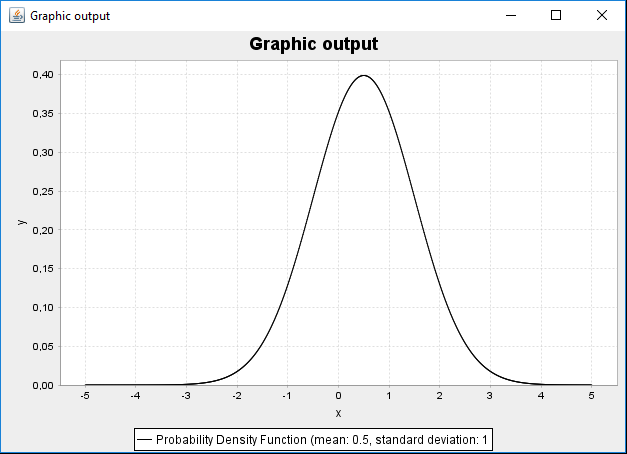
\includegraphics[width=1\textwidth]{Figures/implemented_functions/normal_pdf}~\\
    \caption{Normal Distribution Plot}
    \label{fig:normalDistPlot}
\end{figure}
%!TEX root = ./seminarpaper.tex

\chapter{Implemented Functions}

	This chapter gives an overview about all implemented functions. Figure \ref{fig:OverviewProbabilityDistributions} on page \pageref{fig:OverviewProbabilityDistributions} shows all of them.

	\begin{figure}[h]
		\centering
		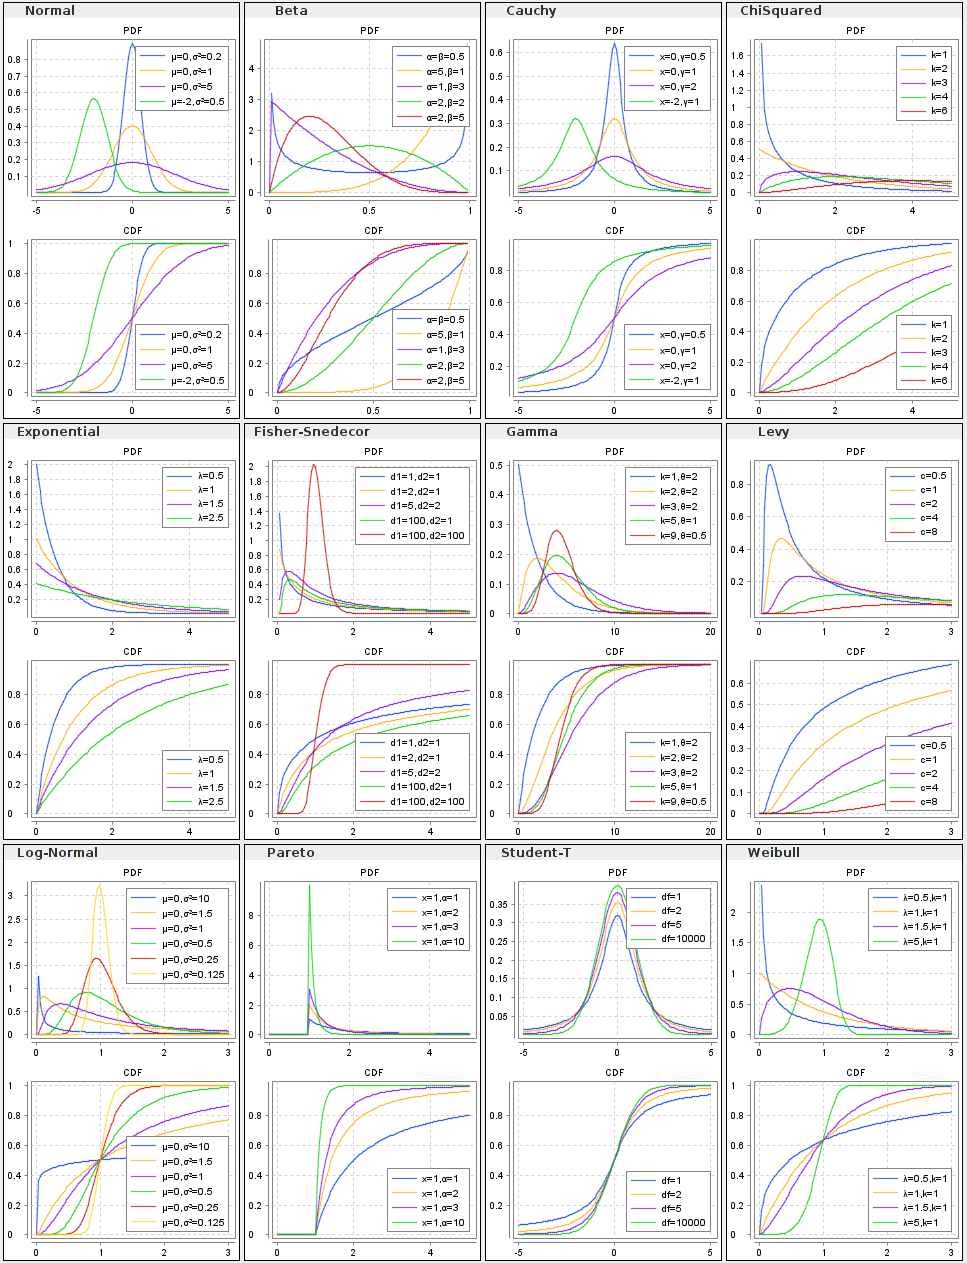
\includegraphics[width=1\textwidth]{Figures/OverviewProbabilityDistributions}~\\
		\caption{Overview Probability Distributions}
		\url{https://commons.apache.org/proper/commons-math/userguide/distribution.html}
		\label{fig:OverviewProbabilityDistributions}
	\end{figure}

	\section{Beta Distribution} \label{sec:beta_distribution}

		The beta distribution has two parameters $\alpha > 0$ and $\beta > 0$ and is defined on the interval $[0,1]$. The \ac{PDF} of the beta distribution is defined as

		$$f(x) = \frac{x^{\alpha-1}(1-x)^{\beta-1}}{B(\alpha,\beta)}  \hspace{.3in} 0 \le x \le 1; \alpha, \beta > 0$$
		\\[0.3cm]		
		with the beta function $B$ as a normalization constant to ensure that the total probability integrates to 1. The formula of the beta function is defined as

		$$B(\alpha,\beta) = \frac{\Gamma(\alpha)\Gamma(\beta)}{\Gamma(\alpha + \beta)}$$
		\\[0.3cm]
		where $\Gamma$ denotes the gamma function. The \ac{CDF} of the beta distribution is defined as

		$$F(x) = I_{x}(\alpha,\beta) = \frac{\int_{0}^{x}{t^{\alpha-1}(1-t)^{\beta-1}dt}}{B(\alpha,\beta)} \hspace{.3in} 0 \le x \le 1; \alpha, \beta > 0$$


	\section{Cauchy Distribution}

		The Cauchy distribution has a location parameter $t$ and a scale parameter $s$ where $s > 0$. The \ac{PDF} of the distribution is defined as

		$$\ds f(x) = \frac{1}{\pi} \cdot \frac{s}{s^2 + (x-t)^2} \quad \hspace{.3in} -\infty<x<\infty$$
		\\[0.3cm]
		The \ac{CDF} is defined as 

		$$\ds F(x) = \frac{1}{2} + \frac{1}{\pi} \cdot \arctan\left(\frac{x-t}{s}\right)$$		

	\section{Chi-squared Distribution}

		The chi-squared distribution (also $\chi^2$-distribution) has only one parameter $k$, where $k \in \mathbb{N}_{>0}$. The \ac{PDF} is defined as

		$$f(x;\,k) =
		\begin{cases}
			\dfrac{x^{(k/2-1)} e^{-x/2}}{2^{k/2} \Gamma\left(\frac k 2 \right)},  & x > 0; \\ 0, & \text{otherwise}.
		\end{cases}$$
		\\[0.3cm]
		where $\Gamma$ is the gamma function. The \ac{CDF} is defined as

		$$F(x;\,k) = \frac{\gamma(\frac{k}{2},\,\frac{x}{2})}{\Gamma(\frac{k}{2})} = P\left(\frac{k}{2},\,\frac{x}{2}\right)$$


	\section{Exponential Distribution}

		The exponential distribution has only the parameter $\lambda$, where $\lambda > 0$. The \ac{PDF} is defined as

		$$f(x;\lambda) = \begin{cases} \lambda e^{-\lambda x} & x \ge 0, \\ 0 & x < 0. \end{cases}$$
		\\[0.3cm]
		The \ac{CDF} is defined as

		$$F(x;\lambda) = \begin{cases} 1-e^{-\lambda x} & x \ge 0 \\ 0 & x < 0. \end{cases}$$

	\section{Fisher-Snedecor Distribution} 

		The Fisher-Snedecor, or F-distribution, has the two parameters $a$ and $b$, where $a,b \in \mathbb{N}_{>0}$. The \ac{PDF} is defined as

		$$
			f(x) = \frac{1}{\mathrm{B}\!\left(\frac{a}{2},\frac{b}{2}\right)} \left(\frac{a}{b}\right)^{\frac{a}{2}} x^{\frac{a}{2} - 1} \left(1+\frac{a}{b}\,x\right)^{-\frac{a+b}{2}}
		$$
		\\[0.3cm]
		where $\Gamma$ denotes the gamma function.
		The \ac{CDF} is defined as

		$$F(x; a,b)=I_{\frac{a x}{a x + b}}\left (\tfrac{a}{2}, \tfrac{b}{2} \right)$$
		\\[0.3cm]
		where $I$ is the regularized incomplete beta function (see section \ref{sec:beta_distribution}).

	\section{Gamma Distribution}

		The gamma distribution has the shape and scale parameters $p$ and $b$, where $p,b > 0$. The \ac{PDF} is defined as

		$$f(x;p,b) =  \frac{x^{p-1}e^{-\frac{x}{b}}}{b^p\Gamma(p)} \quad \text{ for } x > 0 \text{ and } p, b > 0.$$
		\\[0.3cm]
		where $\Gamma(p)$ is a complete \href{https://en.wikipedia.org/wiki/Gamma_function}{gamma function}.		The \ac{CDF} is defined as

		$$F(x;p,b) = \int_0^x f(u;p,b)\,du = \frac{\gamma\left(p, \frac{x}{b}\right)}{\Gamma(p)}$$
		\\[0.3cm]
		where $\gamma\left(p, \frac{x}{b}\right)$ is the lower \href{https://en.wikipedia.org/wiki/Incomplete_gamma_function}{incomplete gamma function}.

	\section{Levy Distribution}

	\section{Log-Normal Distribution}

	\section{Normal Distribution}

	\section{Pareto Distribution}

	\section{Student-T Distribution}
	
		The student distribution has one parameter \nu\ (degrees of freedom) $>$ 0. The \ac{PDF} of the student distribution is defined as
		\\
		$$f(t) = \frac{\Gamma(\frac{\nu+1}{2})} {\sqrt{\nu\pi}\,\Gamma(\frac{\nu}{2})} \left(1+\frac{t^2}{\nu} \right)^{\!-\frac{\nu+1}{2}}$$
		\\
		where $\Gamma$ is the gamma function. The \ac{CDF} of the student distribution can be written in terms of $I$, the regularized incomplete beta function. For $t > 0$
		\\
		$$F(t) = \int_{-\infty}^t f(u)\,du = 1 - \tfrac{1}{2} I_{x(t)}\left(\tfrac{\nu}{2}, \tfrac{1}{2}\right)$$
		\\
		where $$x(t) = \frac{\nu}{{t^2+\nu}}$$

	\section{Weibull Distribution}
	
		The weibull distribution has two parameters $k$ (shape) $>$ 0 and $\gamma$ (scale) $>$ 0 and is defined for \textit{x} \geq\ 0. The \ac{PDF} of the weibull distribution is defined as
		\\
		$$f(x) = \left(\frac{k}{\gamma}\right)\left(\frac{x}{\gamma}\right)^{k-1}e^{-\left(\frac{x}{\gamma}\right)^{k}} \hspace{.3in} x \geq 0; k,\gamma > 0\\$$
		\\
		The \ac{CDF} of the weibull distribution is defined as
		\\
		$$F(x) = 1 - e^{-(x^{\gamma})} \hspace{.3in} x \geq 0; \gamma > 0$$
%!TEX root = ./seminarpaper.tex

\chapter{Testing the Implementation}

	As defined in the task, the values of the statistical distributions implemented in \setlx\ should be tested. Testing should be done in two different ways - integration tests and regression tests. Both tests are described in the sections below.


\section{Integration Tests}

	The \setlx\ interpreter itself has two special test folders, one for regression tests (\lstinline{example_SetlX_code}) and one for integration tests (\lstinline{integrationTests}), containing code of all kinds of tests. Integration tests are tests written in the \setlx\ language, that ensure that implemented functions really exist and that they really deliver the correct solution. The folder for the integration tests is located in the \lstinline{interpreter} folder (listing \ref{lis:integrationTests}). 

	\begin{center}
		\begin{lstlisting}[caption={Path to Integration Tests}, label={lis:integrationTests}]
			setlX
			|-- example_SetlX_code
			`-- interpreter
				|-- integrationTests
				`-- stat_addon
		\end{lstlisting}
	\end{center}

	For the statistical distributions asset a new file \lstinline{stat.stlx} was created inside the \lstinline{integrationTests} folder. This file holds the tests for all 24 implemented distributions. At the beginning of the file, a special file named \lstinline{baseIntegrationTest.stlx} is loaded that will validate the tests. For each distribution, a \setlx\ procedure was written. The following listing shows this with an example. 

	\begin{center}
		\begin{lstlisting}[caption={Test File Example}, language={setlx}, label=lis:exampleCode]
		statChiSquared := procedure() {
			if (stat_chiSquared(2,3) == 0.2075537487102973) {
				correct := true;
			} else {
				print("Error is in: stat_chiSquared(2, 3) == $0.2075537487102973$");
				correct := false;
			}

			validateForTestCase("statChiSquared")
				.that(
					correct
				).is(
					true
				);
		};
		statChiSquared();
		\end{lstlisting}
	\end{center}

	After the procedure is called, the implemented distribution will be called with some parameters. An \lstinline{if} statement checks whether the result of the function call matches the number in the statement. Depending on the result, the test will pass or fail.


\section{Regression Tests}

	Regression tests basically check that everything still works the same. This is especially very important after changes have been done.

	To test all regression tests within the folder, a script named \lstinline{test_all_examples} needs to be executed. The script will first run all integration tests and after validating these tests, the script will check the regression tests, by searching for files that end in \lstinline{.stlx} and files that have the same basename, but end in \lstinline{.stlx.reference}. Once both files are found, the \lstinline{.stlx} file will be executed and the result will be compared with the corresponding \lstinline{.stlx.reference} file, that definitely contains the solution of the \setlx\ program. For the comparison \lstinline{diff} is used. If the result matches the solution, the diff needs to be empty. If so, the next source file will be executed. If not, the script will stop and the result needs to be analyzed.

	The idea was to expand this scheme for the tests of the implemented statistical distributions. Since each asset has its own test folder, it was decided to create a new folder named \lstinline{stat_test_code}, which would then contain all test and reference files. The resulting folder structure of \lstinline{example_SetlX_code} looks like the following:
	
	\begin{center}
		\begin{lstlisting}[caption={Folder Structure \lstinline{example\_SetlX\_code}}, label={lis:regressionTests}]
			example_SetlX_code
			|-- animation_testcode
			|-- converted_Setl2_code
			|-- performance_test_code
			|   `-- results
			|-- plotting_test_code
			|-- simple_examples
			|   `-- gfx_addon
			`-- stat_test_code
		\end{lstlisting}
	\end{center}

	In total 24 statistical distributions were implemented. For each function, a test and a reference file were created, so that there are 48 files in total. All test files follow the same pattern, which is shown in the following listing. The reference files only contain the solution of the program, which would be 0.04405413986167643 in case of the example below.

	\begin{center}
		\begin{lstlisting}[caption={Test File Example}, language={setlx}, label={lis:exampleCode}]
		// Example for stat_normal(x, mu, sigma)

		statNormal := procedure(x, mu, sigma) {

			print(stat_normal(x, mu, sigma));
		};

		x     := 2;
		mu	  := 3;
		sigma := 9;

		statNormal(x, mu, sigma);
		\end{lstlisting}
	\end{center}


\section{Testing with Python}

	In addition to the integration and the regression tests, the computed \setlx\ values should also be compared with values computed with the programming language R or Python. It was decided to test with Python because of existing knowledge. The open-source library \ac{SciPy} was used. \ac{SciPy} provides many user-friendly and efficient numerical routines. More about \ac{SciPy} can be read \href{https://www.scipy.org/}{here}.

	\ac{SciPy} is installed very easily. It basically just needs \lstinline{Python}, \lstinline{Pip}, a package manager from Python, and the \lstinline{SciPy} package itself. However, it is advisable to install \ac{SciPy} in a virtual environment, an isolated Python environment, just for this project. The following commands were executed to install everything needed.

	\begin{center}
		\begin{lstlisting}[caption={Install Virtual Environment and SciPy}, language={bash}, label={lis:scipy}]
			sudo apt-get install python python-pip python-virtualenv virtualenvwrapper
			echo source /usr/share/virtualenvwrapper/virtualenvwrapper.sh >> ~/.bashrc
			source ~/.bashrc
			# Create virtual environment
			mkvirtualenv studienarbeit

			# If virtual environment is activated, execute the following:
			# Update pip
			pip install -U pip
			pip install scipy
		\end{lstlisting}
	\end{center}

	The question was were to save the Python test files. The first idea was to put them into the same folder, were the \setlx\ test files are located. But since this folder only contains tests written in \setlx, it was decided to create a new folder, just for the \enquote{stat} tests. This folder was named \lstinline{example_SetlX_stat_code}. Inside this folder another folder named \lstinline{stat_python_code} was created. In future, if needed, there can be added more folders easily for other tests with other programming languages.

	Once \ac{SciPy} was installed, the test files were created. For each function, there exists one \lstinline{.py} file with the code and one \lstinline{.py.reference} file for the solution - like the tests for \setlx. The listing below shows the test for the normal distribution. Each test file is structured in the same way.

	\begin{center}
		\begin{lstlisting}[caption={Python Test Example}, language={Python}, label={lis:pythontest}]
			from scipy.stats import norm
			print(norm.pdf(2,3,9))
		\end{lstlisting}
	\end{center}

	In line one, the used distribution (\lstinline{norm}) is loaded from the module \ac{SciPy}. Line two calls the \ac{PDF} of the normal distribution and prints the result. The given parameters equal the parameters used in the \setlx\ tests. Calling the \ac{CDF} of any of these distributions works the same way.
%!TEX root = ./seminarpaper.tex

\chapter{Conclusion}

	As developing additional features for \setlx\ was planned by the original developers, the core framework to do so is cleary structured and makes it rather easy to get involved into the matter. Yet it still provides a challenge and is thus well suited as a task for a seminar paper like the one of the authoring students. As this was probably not the last time students develop new features for \setlx\, this document should besides documenting the work of the authors also serve as  an introduction and guide for anyone working on new \setlx\ features.

\chapter*{Abbreviations}
	% \addcontentsline{toc}{chapter}{Abbreviation}
	\begin{acronym}[SciPy]
		\setlength{\itemsep}{-\parsep}
		\acro{CDF}[\textup{CDF}]{cumulative distribution function}
		\acro{PDF}[\textup{PDF}]{probability density function}
		\acro{RSS}[\textup{RSS}]{residual sum of squares}
		\acro{SciPy}[\textup{SciPy}]{Scientific Library for Python}
		\acro{TSS}[\textup{TSS}]{total sum of squares}
	
	\end{acronym}

	
	
\lstlistoflistings



\bibliographystyle{/usr/local/texlive/2015/texmf-dist/bibtex/bst/base/plain.bst}

\bibliography{./cs}
\end{document}

%%% Local Variables:
%%% mode: latex
%%% TeX-master: t
%%% End:
